\subsection{End-to-End Dense Video Captioning with Masked Transformer}

\subsubsection{Overview}

\par Luowei Zhou \textit{et al}, in their 2018 paper titled \textit{End-to-End Dense Video Captioning with Masked Transformer} \cite{zhou2018end}, proposed the problem of \textit{end-to-end training} and \textit{learning long range dependencies} in dense video captioning. Their work highlights the fact that events and captions are closely related. To use language outputs in localizing events, they introduced \textit{end-to-end transformer model with self-attention mechanism}. The network employs a \textit{masking network} which makes the entire training process end-to-end.


\subsubsection{Datasets}
\begin{itemize}
\item YouCook2
\item ActivityNet Captions
\end{itemize}

\subsubsection{Performance}
\par Zhou \textit{et al} compared captioning results with Bi-LSTM + temporal Attention\cite{yao2015describing} using BLEU@3-4 and METEOR. Their work performed better with ground-truth proposals as well as learnt proposals. The proposal generation results were compared to ProcNets\cite{zhou2017automatic}. The average recall of self-attention based mechanism was higher by approximately 6\% than ProcNets.


\subsubsection{Methodology}

\par Zhou \textit{et al} end-to-end model consists of three components:
\begin{enumerate}
	\item Video encoder
	\item Proposal decoder
	\item Captioning decoder with mask prediction network
\end{enumerate}

\begin{figure}[h]
	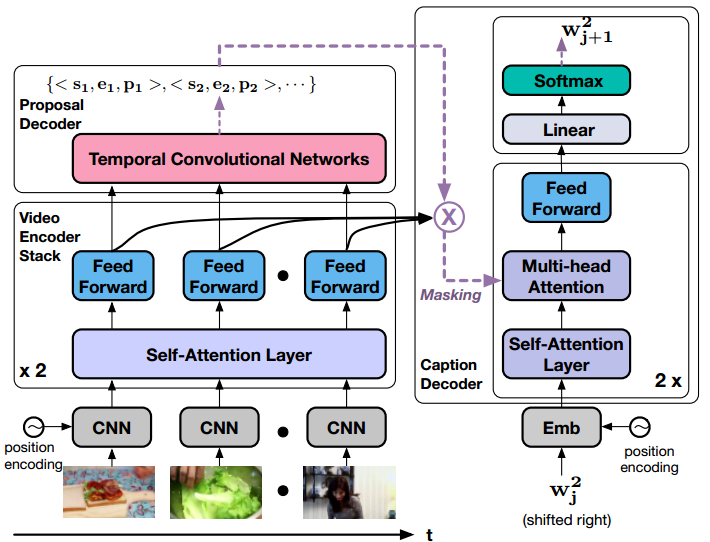
\includegraphics[width=\linewidth]{assets/img/zhou2018end-architecture.png}
	\caption{Masked transformer based architecture introduced by Zhou \textit{et al} (taken from \cite{zhou2018end})}
\end{figure}

\paragraph{End-to-End transformer model}
\begin{enumerate}
	\item L-layered multihead attention on sampled input video frames.
	\item ProcNets\cite{zhou2017automatic} based proposal decoder with following changes:
	\begin{enumerate}
		\item No sequential prediction module.
		\item Bi-LSTM + ResNet encodings replaced with above obtained attention-based encodings.
		\item Multi-layered temporal CNN with variable stride. 
	\end{enumerate}
	\item Caption is generated based on masked features with respect to the proposal boundaries.
\end{enumerate}


\subsubsection{Conclusion}

\par Zhou \textit{et al} presented end-to-end transformer based model for dense video captioning. The network ensures correlation between proposal boundaries and language. They propose to extend their work with object detectors/trackers into current captioning module for better attribution to objects in the scene.